\section{连续分布}
\label{sec:cdist-continuous}

连续模型用密度描述概率：区间上的概率是密度在区间上的积分，任何单点的概率都是零。建立一个连续模型，先确定取值范围，即密度为正的区域，称为支撑；再检查密度非负、在整条实轴上的积分等于一；然后用积分计算期望与方差。积分可能发散，所以每个数值特征都要先核对绝对可积，不能凭对称性或公式的样子直接写出。

连续模型的参数往往分工明确。下面的引理说明，把一个随机变量平移和伸缩，密度怎样跟着变化。一般映射下的密度换算在第~\ref{chap:random-variable-transformations}章统一处理，这里只需要最简单的线性情形。

\begin{lemma}[平移与伸缩]
\label{lem:cdist-location-scale}
设$X$有密度$f_X$，$a\in\mathbb{R}$，$s>0$，令$Y=a+sX$。则$Y$有密度
\begin{equation}
  f_Y(y)=\frac1s\,f_X\Bigl(\frac{y-a}{s}\Bigr).
  \label{eq:cdist-location-scale}
\end{equation}
若$X$的期望存在，则$\mathbb{E}[Y]=a+s\,\mathbb{E}[X]$；若$X$的方差有限，则$\operatorname{Var}(Y)=s^{2}\operatorname{Var}(X)$。
\end{lemma}

\begin{proof}
$s>0$，所以$Y\leq y$与$X\leq(y-a)/s$是同一事件。用$X$的密度写出这个概率，再作代换$u=(v-a)/s$，$\mathrm{d}u=\mathrm{d}v/s$：
\[
  \mathbb{P}(Y\leq y)=\int_{-\infty}^{(y-a)/s}f_X(u)\,\mathrm{d}u
  =\int_{-\infty}^{y}\frac1s\,f_X\Bigl(\frac{v-a}{s}\Bigr)\mathrm{d}v .
\]
这对每个$y$成立，所以式~\eqref{eq:cdist-location-scale}是$Y$的密度。期望与方差的变化规律是第~\ref{chap:random-variable-moments}章的平移与缩放法则。
\end{proof}

许多分布族的成员彼此只差一次平移和伸缩。决定平移量的参数称为\term{位置参数}（location parameter），决定伸缩倍数的参数称为\term{尺度参数}（scale parameter），两者都不改变密度曲线的基本形状。改变形状本身的参数称为\term{形状参数}（shape parameter）。

尺度参数与标准差成正比，但比例系数因分布而异，下面会看到，只有高斯分布的惯用参数恰好等于标准差。因此不能把尺度参数一律当作标准差使用。

\subsection{均匀分布}
\label{sec:cdist-uniform}

公交车每$10$分钟一班，乘客在不知道时刻表的情况下随机到站，等待时间$W$落在$0$到$10$分钟之间。如果没有理由认为哪个时刻到站更多，就应当要求等长的时间段有相等的概率。这个要求把密度确定为区间上的常数。

\begin{definition}[均匀分布]
\label{def:cdist-uniform}
设$a<b$。若随机变量$X$的密度为
\begin{equation}
  f_X(x)=
  \begin{cases}
    \dfrac{1}{b-a}, & a<x<b,\\
    0, & \text{其他},
  \end{cases}
  \label{eq:cdist-uniform-density}
\end{equation}
则称$X$服从区间$(a,b)$上的\term{均匀分布}（uniform distribution），记作$X\sim\operatorname{Unif}(a,b)$。
\end{definition}

密度非负，积分是$(b-a)\cdot\frac{1}{b-a}=1$。对$a\leq c<d\leq b$，概率与区间长度成正比：
\[
  \mathbb{P}(c<X<d)=\frac{d-c}{b-a}.
\]
区间外的概率为零。单点的概率也为零：$\mathbb{P}(X=c)$不超过任何包含$c$的小区间的概率$2\varepsilon/(b-a)$，令$\varepsilon\to0$即得。所以区间写成开的还是闭的，不影响任何概率。

分布函数在$(a,b)$上线性上升，两侧分别为$0$和$1$：
\[
  F_X(x)=
  \begin{cases}
    0, & x\leq a,\\
    (x-a)/(b-a), & a<x<b,\\
    1, & x\geq b.
  \end{cases}
\]

等车的例子中$W\sim\operatorname{Unif}(0,10)$，等待超过$7$分钟的概率是$3/10$，即$1-F_W(7)$，图~\ref{fig:cdist-uniform}的两幅子图分别从密度和分布函数读出这个数。

\begin{BookInlineFigure}
  \centering
  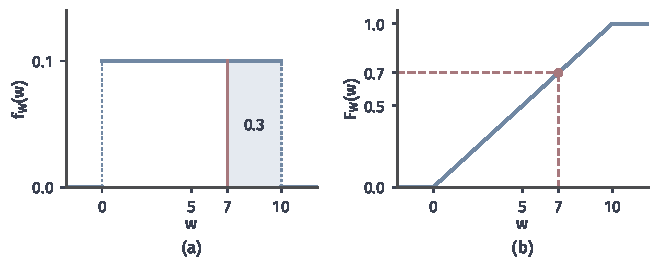
\includegraphics[width=112mm]{figures/07-probability/01-elementary-probability/matplotlib/cdist-uniform/figure.pdf}
  \caption{等待时间$W\sim\operatorname{Unif}(0,10)$。(a)密度，浅蓝面积为$\mathbb{P}(W>7)=0.3$，红线为阈值$7$。(b)分布函数，红点$F_W(7)=0.7$。}
  \label{fig:cdist-uniform}
\end{BookInlineFigure}

\paragraph{期望与方差}
密度关于区间中点对称，期望是中点。直接积分可以验证：
\[
  \mathbb{E}[X]=\frac{1}{b-a}\int_a^bx\,\mathrm{d}x=\frac{b^{2}-a^{2}}{2(b-a)}=\frac{a+b}{2}.
\]
二阶矩为
\[
  \mathbb{E}[X^{2}]=\frac{1}{b-a}\int_a^bx^{2}\,\mathrm{d}x=\frac{b^{3}-a^{3}}{3(b-a)}=\frac{a^{2}+ab+b^{2}}{3}.
\]
减去期望的平方，并把分子通分：
\[
  \operatorname{Var}(X)=\frac{4(a^{2}+ab+b^{2})-3(a+b)^{2}}{12}=\frac{a^{2}-2ab+b^{2}}{12}.
\]
所以
\begin{equation}
  \mathbb{E}[X]=\frac{a+b}{2},\qquad \operatorname{Var}(X)=\frac{(b-a)^{2}}{12}.
  \label{eq:cdist-uniform-moments}
\end{equation}

\paragraph{平移与伸缩}
同一结果可以从$(0,1)$上的均匀分布得到。设$U\sim\operatorname{Unif}(0,1)$，由引理~\ref{lem:cdist-location-scale}，$a+(b-a)U$的密度在$(a,b)$上等于$1/(b-a)$，即$\operatorname{Unif}(a,b)$。$U$的期望为$1/2$、方差为$1/12$，平移不改变方差，伸缩$b-a$倍使方差乘以$(b-a)^{2}$，正好回到式~\eqref{eq:cdist-uniform-moments}。

这里$a$是位置参数，区间长度$b-a$是尺度参数。标准差是$(b-a)/\sqrt{12}\approx0.289(b-a)$，只有区间长度的三成左右。等车的例子中平均等$5$分钟，标准差约$2.89$分钟。

\paragraph{“均匀”需要理由}
均匀分布是一个模型假设，要有“没有位置更特殊”的理由才能采用。乘客若会查看时刻表，到站时刻就集中在发车之前，等待时间不再均匀。均匀分布也只能放在有限区间上：若整条实轴上的密度恒为常数$c$，则$c=0$时积分为零，$c>0$时积分发散，都不能等于一。

\subsection{指数分布}
\label{sec:cdist-exponential}

一台机器在两次故障之间的运行时间$T$是一个连续的等待时间。几何分布描述的是按次计数的等待，这里时间可以取任意正实数。我们希望保留几何分布的无记忆性：已经运行了$s$小时没出故障，剩余时间的分布与新机器相同。下面先给出模型，再说明无记忆性确实把它确定下来。

\begin{definition}[指数分布]
\label{def:cdist-exponential}
设$\lambda>0$。若随机变量$T$的密度为
\begin{equation}
  f_T(t)=\lambda\,\mathrm{e}^{-\lambda t},\quad t\geq0;\qquad f_T(t)=0,\quad t<0,
  \label{eq:cdist-exponential-density}
\end{equation}
则称$T$服从率为$\lambda$的\term{指数分布}（exponential distribution），记作$T\sim\operatorname{Exp}(\lambda)$。参数$\lambda$称为\term{率参数}（rate parameter）。
\end{definition}

密度在$[0,\infty)$上的积分是反常积分，
\[
  \int_0^{\infty}\lambda\,\mathrm{e}^{-\lambda t}\,\mathrm{d}t=\lim_{R\to\infty}\bigl(1-\mathrm{e}^{-\lambda R}\bigr)=1 .
\]
同样的计算给出生存概率，即超过时刻$t$仍在等待的概率：
\begin{equation}
  \mathbb{P}(T>t)=\mathrm{e}^{-\lambda t},\qquad t\geq0 .
  \label{eq:cdist-exponential-survival}
\end{equation}

\paragraph{期望与方差}
各阶矩可以用分部积分逐阶降次。对正整数$k$，在$[0,R]$上分部积分，
\[
  \int_0^{R}t^{k}\lambda\,\mathrm{e}^{-\lambda t}\,\mathrm{d}t
  =-R^{k}\mathrm{e}^{-\lambda R}+\frac{k}{\lambda}\int_0^{R}t^{k-1}\lambda\,\mathrm{e}^{-\lambda t}\,\mathrm{d}t .
\]
$R\to\infty$时边界项趋于零，因为指数衰减快于任何多项式增长；反常积分与分部积分的这些规则可参考\BookChapterRef{chap:univariate-integration}{卷一第7章“一元函数的积分”}。于是
\[
  \mathbb{E}[T^{k}]=\frac{k}{\lambda}\,\mathbb{E}[T^{k-1}],
\]
从$\mathbb{E}[T^{0}]=1$递推得
\begin{equation}
  \mathbb{E}[T^{k}]=\frac{k!}{\lambda^{k}},\qquad k=0,1,2,\dots .
  \label{eq:cdist-exponential-moments-k}
\end{equation}

取$k=1,2$，再用方差的展开式，得到
\begin{equation}
  \mathbb{E}[T]=\frac1\lambda,\qquad \operatorname{Var}(T)=\frac{2}{\lambda^{2}}-\frac{1}{\lambda^{2}}=\frac{1}{\lambda^{2}}.
  \label{eq:cdist-exponential-moments}
\end{equation}
率$\lambda$是单位时间内的平均事件数，均值$1/\lambda$是平均等待时间。$1/\lambda$是尺度参数：$\lambda T\sim\operatorname{Exp}(1)$。指数分布的标准差恰好等于均值。

设机器的故障率为每小时$0.5$次，即$T\sim\operatorname{Exp}(0.5)$。平均运行$2$小时，标准差也是$2$小时，运行超过$3$小时的概率是$\mathrm{e}^{-1.5}\approx0.223$。中位数$m$满足$\mathrm{e}^{-0.5m}=1/2$，即$m=2\ln2\approx1.39$小时，比均值小：少数很长的运行时间把均值拉向右侧。

\paragraph{无记忆性}
已经运行了$s$小时，再运行$t$小时以上的条件概率为
\[
  \mathbb{P}(T>s+t\mid T>s)=\frac{\mathrm{e}^{-\lambda(s+t)}}{\mathrm{e}^{-\lambda s}}=\mathrm{e}^{-\lambda t}=\mathbb{P}(T>t).
\]
例如已经运行$1$小时，再运行$3$小时以上的概率仍是$0.223$，与新机器一样。这里同样用到$\{T>s+t\}\subseteq\{T>s\}$。

与离散情形一样，无记忆性在有密度的非负变量中只属于指数分布。

\begin{theorem}[指数分布的无记忆刻画]
\label{thm:cdist-exponential-memoryless}
设$T$取非负值且有密度，对每个$t\geq0$有$\mathbb{P}(T>t)>0$。若对所有$s,t\geq0$都有
\begin{equation}
  \mathbb{P}(T>s+t\mid T>s)=\mathbb{P}(T>t),
  \label{eq:cdist-memoryless-continuous}
\end{equation}
则存在$\lambda>0$使$T\sim\operatorname{Exp}(\lambda)$。
\end{theorem}

\begin{proof}
记$G(t)=\mathbb{P}(T>t)$。$T$有密度，单点概率为零，所以$G(0)=1$。式~\eqref{eq:cdist-memoryless-continuous}即
\[
  G(s+t)=G(s)G(t),\qquad s,t\geq0 .
\]

先看有理点。对正整数$k,m$，反复使用上式得$G(k/m)=G(1/m)^{k}$，特别地$G(1)=G(1/m)^{m}$。记$c=G(1)>0$，则$G(1/m)=c^{1/m}$，从而
\[
  G(r)=c^{r},\qquad r\text{为正有理数}.
\]

再说明$c<1$。$G(n)=\int_n^{\infty}f_T(u)\,\mathrm{d}u$是收敛反常积分的尾部，$n\to\infty$时趋于零；而$G(n)=c^{n}$，所以$c<1$。

最后看一般的$t>0$。$G$是非增函数，对有理数$r<t<r'$有$c^{r'}\leq G(t)\leq c^{r}$。令$r$与$r'$都趋于$t$，由$r\mapsto c^{r}$的连续性得$G(t)=c^{t}$。令$\lambda=-\ln c>0$，则$G(t)=\mathrm{e}^{-\lambda t}$。生存概率决定分布函数，与式~\eqref{eq:cdist-exponential-survival}比较即知$T\sim\operatorname{Exp}(\lambda)$。
\end{proof}

\paragraph{与几何分布的联系}
指数分布与几何分布可以互相转化。把$T\sim\operatorname{Exp}(\lambda)$向上取整，记$\lceil T\rceil$为运行过的整小时数。对整数$k\geq0$，$\lceil T\rceil>k$与$T>k$是同一事件，所以
\[
  \mathbb{P}(\lceil T\rceil>k)=\mathrm{e}^{-\lambda k}=\bigl(\mathrm{e}^{-\lambda}\bigr)^{k}.
\]
与式~\eqref{eq:cdist-geometric-tail}比较，$\lceil T\rceil\sim\operatorname{Geom}(1-\mathrm{e}^{-\lambda})$。

反过来，把时间切成长为$h$的小段，每段以概率$\lambda h$发生故障，各段独立。等到故障的段数$T_h\sim\operatorname{Geom}(\lambda h)$，等待时间约为$hT_h$。对固定的$t>0$，
\[
  \mathbb{P}(hT_h>t)=(1-\lambda h)^{\lfloor t/h\rfloor}.
\]
取对数，$\lfloor t/h\rfloor$与$t/h$相差不到$1$，而$\ln(1-\lambda h)/h\to-\lambda$，所以上式在$h\to0$时趋于$\mathrm{e}^{-\lambda t}$。指数分布是几何等待在时间连续化之后的极限，见图~\ref{fig:cdist-exponential-geometric}(b)。

\begin{BookInlineFigure}
  \centering
  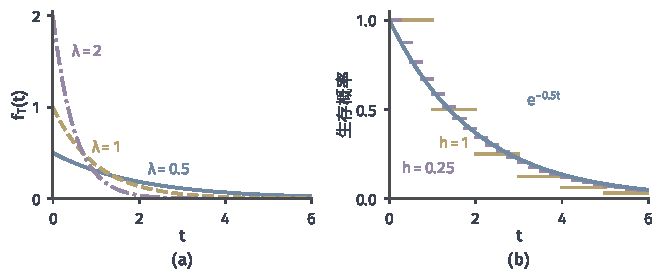
\includegraphics[width=112mm]{figures/07-probability/01-elementary-probability/matplotlib/cdist-exponential-geometric/figure.pdf}
  \caption{指数分布。(a)率$\lambda=0.5$（蓝）、$1$（黄）、$2$（紫）的密度，均值分别为$2,1,0.5$。(b)$\operatorname{Exp}(0.5)$的生存概率$\mathrm{e}^{-0.5t}$（蓝），以及每段长$h$、每段发生概率$0.5h$的几何等待的生存概率：$h=1$（黄）和$h=0.25$（紫）的阶梯随$h$变小贴近蓝线。}
  \label{fig:cdist-exponential-geometric}
\end{BookInlineFigure}

两者的区别也要记清。几何分布取正整数，每个值都有正概率，无记忆性只在整数步上成立；指数分布取连续值，单点概率为零，无记忆性对任意实数$s,t$成立。几何分布的参数$p$是每次试验的概率，不超过$1$；指数分布的$\lambda$是单位时间的率，可以是任意正数，量纲为时间的倒数。

\subsection{高斯分布}
\label{sec:cdist-gaussian}

零件长度的测量值总在标称值附近波动：靠近中心的偏差最常见，偏差越大越少见，正负两侧对称。这样的误差往往是许多微小扰动叠加的结果，它们的和近似服从钟形的分布，第~\ref{chap:central-limit-theorem}章会在明确的条件下证明这一点。这里把钟形密度当作给定的模型，研究它的归一化、参数和区间概率。

钟形由$\mathrm{e}^{-z^{2}/2}$给出。要把它变成密度，先得算出它在整条实轴上的积分。

\begin{lemma}[Gauss积分]
\label{lem:cdist-gauss-integral}
反常积分$\int_{-\infty}^{\infty}\mathrm{e}^{-z^{2}/2}\,\mathrm{d}z$收敛，并且
\begin{equation}
  \int_{-\infty}^{\infty}\mathrm{e}^{-z^{2}/2}\,\mathrm{d}z=\sqrt{2\pi}.
  \label{eq:cdist-gauss-integral}
\end{equation}
\end{lemma}

\begin{proof}
由$(\lvert z\rvert-1)^{2}\geq0$得$z^{2}/2\geq\lvert z\rvert-1/2$，所以被积函数不超过$\mathrm{e}^{1/2}\mathrm{e}^{-\lvert z\rvert}$，积分收敛。记$I_R$为被积函数在$[-R,R]$上的积分，它的平方是正方形$Q_R=[-R,R]^{2}$上的二重积分：
\[
  I_R^{2}=\iint_{Q_R}\mathrm{e}^{-(x^{2}+y^{2})/2}\,\mathrm{d}x\,\mathrm{d}y .
\]

在圆盘上，这个二重积分可以用极坐标算出来。对半径为$\rho$的圆盘$D_\rho$，面积权重为$r$，于是
\[
  \iint_{D_\rho}\mathrm{e}^{-(x^{2}+y^{2})/2}\,\mathrm{d}x\,\mathrm{d}y
  =\int_0^{2\pi}\!\!\int_0^{\rho}\mathrm{e}^{-r^{2}/2}\,r\,\mathrm{d}r\,\mathrm{d}\theta
  =2\pi\bigl(1-\mathrm{e}^{-\rho^{2}/2}\bigr).
\]
极坐标换元可参考\BookChapterRef{chap:region-integrals}{卷二第24章“区域积分”}。

正方形夹在两个圆盘之间：$D_R\subseteq Q_R\subseteq D_{\sqrt2R}$。被积函数为正，区域越大积分越大，所以
\[
  2\pi\bigl(1-\mathrm{e}^{-R^{2}/2}\bigr)\leq I_R^{2}\leq2\pi\bigl(1-\mathrm{e}^{-R^{2}}\bigr).
\]
令$R\to\infty$，两端都趋于$2\pi$，故$I_R^{2}\to2\pi$。$I_R$为正，所以极限是$\sqrt{2\pi}$。
\end{proof}

\begin{definition}[高斯分布]
\label{def:cdist-gaussian}
密度为
\begin{equation}
  \varphi(z)=\frac{1}{\sqrt{2\pi}}\,\mathrm{e}^{-z^{2}/2},\qquad z\in\mathbb{R},
  \label{eq:cdist-standard-gaussian}
\end{equation}
的分布称为\term{标准高斯分布}（standard Gaussian distribution），记作$\mathcal{N}(0,1)$。设$\mu\in\mathbb{R}$，$\sigma>0$。若随机变量$X$的密度为
\begin{equation}
  f_X(x)=\frac{1}{\sqrt{2\pi}\,\sigma}\exp\Bigl(-\frac{(x-\mu)^{2}}{2\sigma^{2}}\Bigr),\qquad x\in\mathbb{R},
  \label{eq:cdist-gaussian-density}
\end{equation}
则称$X$服从\term{高斯分布}（Gaussian distribution），也称正态分布，记作$X\sim\mathcal{N}(\mu,\sigma^{2})$。
\end{definition}

由引理~\ref{lem:cdist-gauss-integral}，$\varphi$的积分为一。比较式~\eqref{eq:cdist-gaussian-density}与式~\eqref{eq:cdist-location-scale}可知，$f_X$正是$\mu+\sigma Z$的密度，其中$Z\sim\mathcal{N}(0,1)$；所以$f_X$的积分也为一。$\mu$是位置参数，$\sigma$是尺度参数：前者平移钟形，后者把它横向拉宽$\sigma$倍、纵向压低$\sigma$倍，见图~\ref{fig:cdist-gaussian}(a)。

\paragraph{期望与方差}
先看标准情形。$\lvert z\rvert\varphi(z)$可积，因为
\[
  \int_0^{\infty}z\,\mathrm{e}^{-z^{2}/2}\,\mathrm{d}z=\Bigl[-\mathrm{e}^{-z^{2}/2}\Bigr]_0^{\infty}=1 .
\]
期望存在，而$z\varphi(z)$是奇函数，两侧相消，所以$\mathbb{E}[Z]=0$。

二阶矩用分部积分。注意$\varphi'(z)=-z\varphi(z)$，把$z^{2}\varphi(z)$写成$z\cdot z\varphi(z)=-z\varphi'(z)$，在$[-R,R]$上分部积分：
\[
  \int_{-R}^{R}z^{2}\varphi(z)\,\mathrm{d}z=\Bigl[-z\varphi(z)\Bigr]_{-R}^{R}+\int_{-R}^{R}\varphi(z)\,\mathrm{d}z .
\]
边界项等于$-2R\varphi(R)$，$R\to\infty$时趋于零，第二项趋于$1$。所以$\mathbb{E}[Z^{2}]=1$，$\operatorname{Var}(Z)=1$。

一般情形由引理~\ref{lem:cdist-location-scale}得到：
\begin{equation}
  \mathbb{E}[X]=\mu,\qquad \operatorname{Var}(X)=\sigma^{2}.
  \label{eq:cdist-gaussian-moments}
\end{equation}
高斯分布的尺度参数$\sigma$恰好是标准差，这是参数化方式带来的巧合，后面的分布都不是这样。

同样的分部积分给出更高阶的矩：$\mathbb{E}[Z^{k+2}]=(k+1)\mathbb{E}[Z^{k}]$，所以$\mathbb{E}[Z^{4}]=3$，奇数阶矩为零。按第~\ref{chap:random-variable-moments}章的定义，高斯分布的偏度为$0$，峰度为$3$，超额峰度约定以它为零点。

\paragraph{区间概率}
标准高斯分布的分布函数记作
\[
  \Phi(z)=\int_{-\infty}^{z}\varphi(u)\,\mathrm{d}u .
\]
它没有初等函数表示，数值要查表或用数值方法算。对称性给出$\Phi(-z)=1-\Phi(z)$，于是只需$z\geq0$的值。几个常用的值是
\[
  \Phi(1)\approx0.8413,\qquad \Phi(1.96)\approx0.9750,\qquad \Phi(2)\approx0.9772 .
\]

一般的$X\sim\mathcal{N}(\mu,\sigma^{2})$先标准化：$X\leq x$等价于$(X-\mu)/\sigma\leq(x-\mu)/\sigma$，而$(X-\mu)/\sigma\sim\mathcal{N}(0,1)$。所以
\begin{equation}
  \mathbb{P}(a<X\leq b)=\Phi\Bigl(\frac{b-\mu}{\sigma}\Bigr)-\Phi\Bigl(\frac{a-\mu}{\sigma}\Bigr).
  \label{eq:cdist-gaussian-interval}
\end{equation}
特别地，落在均值左右$k$个标准差以内的概率是$2\Phi(k)-1$，$k=1,2,3$时依次为
\[
  0.6827,\qquad 0.9545,\qquad 0.9973 .
\]

设零件长度$X\sim\mathcal{N}(10,0.2^{2})$，单位为毫米，合格范围是$[9.8,10.4]$。上下限分别在均值右侧两个标准差和左侧一个标准差处，由式~\eqref{eq:cdist-gaussian-interval}，
\[
  \mathbb{P}(9.8\leq X\leq10.4)=\Phi(2)-\bigl(1-\Phi(1)\bigr)\approx0.9772-0.1587\approx0.819 .
\]
合格范围不对称，所以合格率不能用“$\pm2\sigma$内$95\%$”之类的口诀套算，图~\ref{fig:cdist-gaussian}(b)标出了这块面积。

\begin{BookInlineFigure}
  \centering
  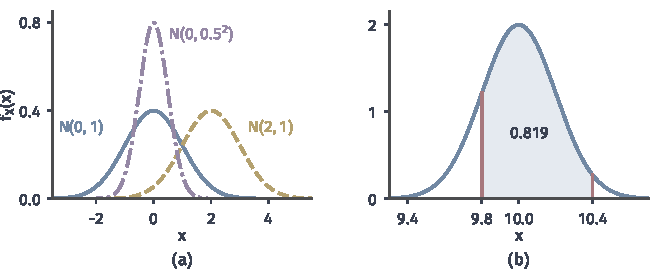
\includegraphics[width=112mm]{figures/07-probability/01-elementary-probability/matplotlib/cdist-gaussian/figure.pdf}
  \caption{高斯分布。(a)$\mathcal{N}(0,1)$（蓝）、平移后的$\mathcal{N}(2,1)$（黄）和尺度减半的$\mathcal{N}(0,0.5^{2})$（紫）。(b)零件长度$\mathcal{N}(10,0.2^{2})$，红线为合格范围的上下限$9.8$与$10.4$（毫米），浅蓝面积为合格率$0.819$。}
  \label{fig:cdist-gaussian}
\end{BookInlineFigure}

\paragraph{尾部}
高斯分布的尾部衰减得极快。对$z>0$，在积分中把$\varphi(u)$放大为$(u/z)\varphi(u)$（因为$u\geq z$），而$u\varphi(u)$有原函数$-\varphi(u)$，得到
\begin{equation}
  1-\Phi(z)\leq\int_z^{\infty}\frac{u}{z}\varphi(u)\,\mathrm{d}u=\frac{\varphi(z)}{z},\qquad z>0 .
  \label{eq:cdist-gaussian-tail}
\end{equation}
尾概率按$\mathrm{e}^{-z^{2}/2}$的速度下降。$z=2$时右端为$0.0270$，真值为$0.0228$；$z=5$时尾概率已不到$3\times10^{-7}$。

这一性质也提醒我们模型的边界。按$\mathcal{N}(10,0.2^{2})$，零件长度为负的概率是$\Phi(-50)$，小到可以忽略，但并不为零；高斯分布在这里是一个近似，并不意味着长度真的可以为负。实际误差若偶尔出现很大的偏离，高斯尾部会严重低估它们的频率，后面的t分布和Laplace分布就是为此准备的。

\subsection{Gamma分布}
\label{sec:cdist-gamma}

指数分布只有一种形状：密度在$0$处最高，然后单调下降。等待第二次、第三次故障的总时间，或者某些只取正值且有偏斜的量，密度往往从零开始先升后降。在指数密度前乘一个幂函数，得到形如$x^{\alpha-1}\mathrm{e}^{-\beta x}$的密度，形状就可以调节。归一化常数需要一个新的函数。

\begin{definition}[Gamma函数]
\label{def:cdist-gamma-function}
对$\alpha>0$，定义
\begin{equation}
  \Gamma(\alpha)=\int_0^{\infty}x^{\alpha-1}\mathrm{e}^{-x}\,\mathrm{d}x .
  \label{eq:cdist-gamma-function}
\end{equation}
称为\term{Gamma函数}（Gamma function）。
\end{definition}

这个反常积分在两端都需要检查。在$0$附近，$x^{\alpha-1}\mathrm{e}^{-x}\leq x^{\alpha-1}$，而$\int_0^1x^{\alpha-1}\,\mathrm{d}x$恰在$\alpha>0$时收敛。在无穷远处，$x^{\alpha-1}\mathrm{e}^{-x/2}$有界，所以被积函数不超过某个常数乘$\mathrm{e}^{-x/2}$，积分收敛。$\alpha\leq0$时$0$附近发散，所以定义要求$\alpha>0$。

\begin{lemma}[Gamma函数的递推]
\label{lem:cdist-gamma-recursion}
对$\alpha>0$，
\begin{equation}
  \Gamma(\alpha+1)=\alpha\,\Gamma(\alpha).
  \label{eq:cdist-gamma-recursion}
\end{equation}
特别地，$\Gamma(1)=1$，对正整数$n$有$\Gamma(n)=(n-1)!$，并且$\Gamma(1/2)=\sqrt\pi$。
\end{lemma}

\begin{proof}
在$[\varepsilon,R]$上分部积分：
\[
  \int_{\varepsilon}^{R}x^{\alpha}\mathrm{e}^{-x}\,\mathrm{d}x
  =\Bigl[-x^{\alpha}\mathrm{e}^{-x}\Bigr]_{\varepsilon}^{R}+\alpha\int_{\varepsilon}^{R}x^{\alpha-1}\mathrm{e}^{-x}\,\mathrm{d}x .
\]
$\varepsilon\to0$、$R\to\infty$时边界项趋于零，即得递推式。$\Gamma(1)$是$\mathrm{e}^{-x}$在$[0,\infty)$上的积分，等于$1$；由递推，$\Gamma(n)=(n-1)\Gamma(n-1)=\dots=(n-1)!$。

对$\Gamma(1/2)$作代换$x=z^{2}/2$，$\mathrm{d}x=z\,\mathrm{d}z$，$x^{-1/2}=\sqrt2/z$：
\[
  \Gamma\Bigl(\frac12\Bigr)=\int_0^{\infty}\frac{\sqrt2}{z}\,\mathrm{e}^{-z^{2}/2}\,z\,\mathrm{d}z=\sqrt2\int_0^{\infty}\mathrm{e}^{-z^{2}/2}\,\mathrm{d}z .
\]
由引理~\ref{lem:cdist-gauss-integral}和对称性，最后的积分是$\sqrt{2\pi}/2$，所以$\Gamma(1/2)=\sqrt\pi$。
\end{proof}

递推式说明Gamma函数把阶乘从正整数延拓到了正实数，图~\ref{fig:cdist-gamma-function}在整数点标出了阶乘。由递推还可以得到半整数处的值，例如$\Gamma(3/2)=\sqrt\pi/2$。

\begin{BookInlineFigure}
  \centering
  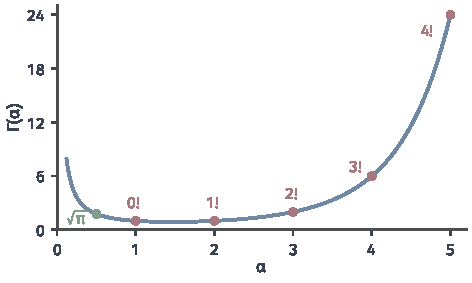
\includegraphics[width=80mm]{figures/07-probability/01-elementary-probability/matplotlib/cdist-gamma-function/figure.pdf}
  \caption{Gamma函数在$(0,5]$上的图像。红点为整数点$\Gamma(n)=(n-1)!$，绿点为$\Gamma(1/2)=\sqrt\pi$。$\alpha\to0^{+}$时$\Gamma(\alpha)\to\infty$。}
  \label{fig:cdist-gamma-function}
\end{BookInlineFigure}

\begin{definition}[Gamma分布]
\label{def:cdist-gamma}
设$\alpha>0$，$\beta>0$。若随机变量$X$的密度为
\begin{equation}
  f_X(x)=\frac{\beta^{\alpha}}{\Gamma(\alpha)}\,x^{\alpha-1}\mathrm{e}^{-\beta x},\quad x>0;\qquad f_X(x)=0,\quad x\leq0,
  \label{eq:cdist-gamma-density}
\end{equation}
则称$X$服从形状为$\alpha$、率为$\beta$的\term{Gamma分布}（Gamma distribution），记作$X\sim\operatorname{Gamma}(\alpha,\beta)$。
\end{definition}

归一化只需一次代换$y=\beta x$：
\[
  \int_0^{\infty}\frac{\beta^{\alpha}}{\Gamma(\alpha)}x^{\alpha-1}\mathrm{e}^{-\beta x}\,\mathrm{d}x
  =\frac{1}{\Gamma(\alpha)}\int_0^{\infty}y^{\alpha-1}\mathrm{e}^{-y}\,\mathrm{d}y=1 .
\]
$\alpha=1$时密度为$\beta\mathrm{e}^{-\beta x}$，就是$\operatorname{Exp}(\beta)$。

\paragraph{期望与方差}
同样的代换给出各阶矩。对$k>-\alpha$，
\[
  \mathbb{E}[X^{k}]=\frac{\beta^{\alpha}}{\Gamma(\alpha)}\int_0^{\infty}x^{\alpha+k-1}\mathrm{e}^{-\beta x}\,\mathrm{d}x
  =\frac{\Gamma(\alpha+k)}{\Gamma(\alpha)\,\beta^{k}} .
\]
取$k=1,2$并用递推式~\eqref{eq:cdist-gamma-recursion}，得到$\mathbb{E}[X]=\alpha/\beta$与$\mathbb{E}[X^{2}]=\alpha(\alpha+1)/\beta^{2}$。于是
\begin{equation}
  \mathbb{E}[X]=\frac{\alpha}{\beta},\qquad \operatorname{Var}(X)=\frac{\alpha(\alpha+1)-\alpha^{2}}{\beta^{2}}=\frac{\alpha}{\beta^{2}}.
  \label{eq:cdist-gamma-moments}
\end{equation}
所有正阶矩都有限。

\paragraph{形状}
形状参数$\alpha$决定密度在$0$附近的行为。$\alpha<1$时$x^{\alpha-1}\to\infty$，密度在$0$处无界，但仍然可积；$\alpha=1$时密度在$0$处取有限正值；$\alpha>1$时密度从$0$出发先升后降。对数导数为$(\alpha-1)/x-\beta$，所以$\alpha>1$时众数为$(\alpha-1)/\beta$。$\alpha$越大，钟形越对称，图~\ref{fig:cdist-gamma-shapes}(a)画出了这几种情形。

$\beta$是率参数，$1/\beta$是尺度参数：由引理~\ref{lem:cdist-location-scale}，$\beta X\sim\operatorname{Gamma}(\alpha,1)$。改变$\beta$只把同一形状横向伸缩。

\begin{BookInlineFigure}
  \centering
  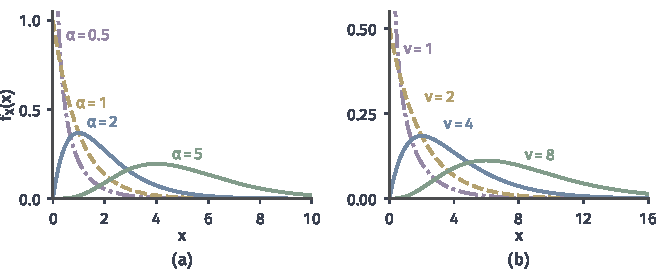
\includegraphics[width=112mm]{figures/07-probability/01-elementary-probability/matplotlib/cdist-gamma-shapes/figure.pdf}
  \caption{Gamma分布的形状。(a)率$\beta=1$，形状$\alpha=0.5$（紫，$0$处无界）、$1$（黄，即$\operatorname{Exp}(1)$）、$2$（蓝）、$5$（绿）。(b)卡方分布$\chi^{2}_{\nu}=\operatorname{Gamma}(\nu/2,1/2)$，$\nu=1,2,4,8$，配色同(a)。}
  \label{fig:cdist-gamma-shapes}
\end{BookInlineFigure}

设故障率为每小时$0.5$次。等待第二次故障的时间$X$常用形状$\alpha=2$、率$\beta=0.5$的Gamma分布描述；它为什么是两段独立指数等待之和的分布，第~\ref{chap:random-variable-transformations}章会给出证明。期望为$4$小时，方差为$8$，众数为$2$小时。超过$4$小时的概率由分部积分算出：
\[
  \mathbb{P}(X>4)=\int_4^{\infty}\frac{x}{4}\,\mathrm{e}^{-x/2}\,\mathrm{d}x
  =\Bigl[-\frac{x}{2}\mathrm{e}^{-x/2}-\mathrm{e}^{-x/2}\Bigr]_4^{\infty}=3\mathrm{e}^{-2}\approx0.406 .
\]

\paragraph{率与尺度两种写法}
不少文献改用尺度$\theta=1/\beta$作参数，密度写成
\[
  f_X(x)=\frac{1}{\Gamma(\alpha)\,\theta^{\alpha}}\,x^{\alpha-1}\mathrm{e}^{-x/\theta},\qquad x>0,
\]
此时期望为$\alpha\theta$，方差为$\alpha\theta^{2}$。同一个记号$\operatorname{Gamma}(2,0.5)$，按率理解期望是$4$，按尺度理解期望是$1$，相差四倍。本卷一律使用率$\beta$。还要注意标准差是$\sqrt\alpha\,\theta$，只有$\alpha=1$时才等于尺度$\theta$。

\paragraph{卡方分布}
Gamma族中有一个特例经常单独出现。对$\nu>0$，形状为$\nu/2$、率为$1/2$的Gamma分布称为自由度为$\nu$的\term{卡方分布}（chi-squared distribution），记作$\chi^{2}_{\nu}$。由式~\eqref{eq:cdist-gamma-moments}，
\begin{equation}
  \mathbb{E}[X]=\nu,\qquad \operatorname{Var}(X)=2\nu,\qquad X\sim\chi^{2}_{\nu}.
  \label{eq:cdist-chisq-moments}
\end{equation}
名称中的“平方”来自它的构造：$\nu$为正整数时，$\nu$个相互独立的标准高斯变量的平方和服从$\chi^{2}_{\nu}$，这一结论在第~\ref{chap:random-variable-transformations}章证明。这里的定义对任意正实数$\nu$都有意义。

\subsection{Beta分布}
\label{sec:cdist-beta}

一批货中次品所占的比例、一次投篮的命中率，都是落在$0$与$1$之间的量。若这些比例本身随批次而变，就需要$(0,1)$上的分布来描述。仿照Gamma分布，在两个端点各放一个幂函数，得到形如$x^{a-1}(1-x)^{b-1}$的密度，两个指数分别控制密度在$0$和$1$附近的行为。为避免与Gamma分布的率$\beta$混淆，这里的参数记作$a,b$。

\begin{definition}[Beta函数与Beta分布]
\label{def:cdist-beta}
对$a>0$，$b>0$，称
\begin{equation}
  \mathrm{B}(a,b)=\int_0^{1}x^{a-1}(1-x)^{b-1}\,\mathrm{d}x
  \label{eq:cdist-beta-function}
\end{equation}
为\term{Beta函数}（Beta function）。若随机变量$X$的密度为
\begin{equation}
  f_X(x)=\frac{x^{a-1}(1-x)^{b-1}}{\mathrm{B}(a,b)},\quad 0<x<1;\qquad f_X(x)=0,\quad\text{其他},
  \label{eq:cdist-beta-density}
\end{equation}
则称$X$服从\term{Beta分布}（Beta distribution），记作$X\sim\operatorname{Beta}(a,b)$。
\end{definition}

积分~\eqref{eq:cdist-beta-function}在$0$附近的被积函数与$x^{a-1}$同阶，在$1$附近与$(1-x)^{b-1}$同阶，所以恰在$a>0$且$b>0$时收敛。密度的归一化由定义直接保证，计算期望和方差则需要Beta函数的两条性质。

\begin{lemma}[Beta函数的性质]
\label{lem:cdist-beta-function}
对$a,b>0$，
\begin{equation}
  \mathrm{B}(a+1,b)=\frac{a}{a+b}\,\mathrm{B}(a,b),
  \label{eq:cdist-beta-recursion}
\end{equation}
并且
\begin{equation}
  \mathrm{B}(a,b)=\frac{\Gamma(a)\,\Gamma(b)}{\Gamma(a+b)} .
  \label{eq:cdist-beta-gamma}
\end{equation}
\end{lemma}

\begin{proof}
先证递推式。被积函数乘以$x+(1-x)=1$再拆开，得到
\[
  \mathrm{B}(a,b)=\mathrm{B}(a+1,b)+\mathrm{B}(a,b+1).
\]
另一方面，对$\mathrm{B}(a+1,b)$分部积分，把$(1-x)^{b-1}$积成$-(1-x)^{b}/b$，边界项在两端为零：
\[
  \begin{aligned}
  \mathrm{B}(a+1,b)&=\int_0^{1}x^{a}(1-x)^{b-1}\,\mathrm{d}x\\
  &=\frac{a}{b}\int_0^{1}x^{a-1}(1-x)^{b}\,\mathrm{d}x=\frac{a}{b}\,\mathrm{B}(a,b+1).
  \end{aligned}
\]
把$\mathrm{B}(a,b+1)=\frac{b}{a}\mathrm{B}(a+1,b)$代入第一式，得到
\[
  \mathrm{B}(a,b)=\Bigl(1+\frac{b}{a}\Bigr)\mathrm{B}(a+1,b)=\frac{a+b}{a}\,\mathrm{B}(a+1,b),
\]
即式~\eqref{eq:cdist-beta-recursion}。

再证式~\eqref{eq:cdist-beta-gamma}。把两个Gamma积分之积写成第一象限上的二重积分：
\[
  \Gamma(a)\Gamma(b)=\int_0^{\infty}\!\!\int_0^{\infty}x^{a-1}y^{b-1}\mathrm{e}^{-(x+y)}\,\mathrm{d}x\,\mathrm{d}y .
\]
被积函数为正，这一步以及下面的换元都可以先在有界区域上进行，再令区域扩大取极限。

作代换$x=st$，$y=s(1-t)$，其中$s>0$，$0<t<1$。它把$(0,\infty)\times(0,1)$一一映到第一象限，逆映射为$s=x+y$，$t=x/(x+y)$。Jacobian行列式为
\[
  \det\begin{pmatrix}t & s\\ 1-t & -s\end{pmatrix}=-ts-s(1-t)=-s,
\]
绝对值为$s$。代入后被积函数分离成$s$的函数与$t$的函数之积：
\[
  \Gamma(a)\Gamma(b)=\int_0^{\infty}s^{a+b-1}\mathrm{e}^{-s}\,\mathrm{d}s\int_0^{1}t^{a-1}(1-t)^{b-1}\,\mathrm{d}t
  =\Gamma(a+b)\,\mathrm{B}(a,b).
\]
\end{proof}

\paragraph{期望与方差}
期望是两个Beta函数之比，由式~\eqref{eq:cdist-beta-recursion}，
\[
  \mathbb{E}[X]=\frac{\mathrm{B}(a+1,b)}{\mathrm{B}(a,b)}=\frac{a}{a+b}.
\]
二阶矩连用两次递推，第二次的参数是$(a+1,b)$：
\[
  \mathbb{E}[X^{2}]=\frac{\mathrm{B}(a+2,b)}{\mathrm{B}(a,b)}=\frac{a+1}{a+b+1}\cdot\frac{a}{a+b}.
\]
减去期望的平方并通分，分子化为$a[(a+1)(a+b)-a(a+b+1)]=ab$，所以
\begin{equation}
  \mathbb{E}[X]=\frac{a}{a+b},\qquad \operatorname{Var}(X)=\frac{ab}{(a+b)^{2}(a+b+1)} .
  \label{eq:cdist-beta-moments}
\end{equation}

\paragraph{端点形状}
参数$a$管左端，$b$管右端。$a<1$时密度在$0$附近无界，$a=1$时在$0$处取有限正值$b$，$a>1$时在$0$处为零；$b$对右端同理。几个特殊情形一目了然：$\operatorname{Beta}(1,1)$就是$\operatorname{Unif}(0,1)$；$a=b$时密度关于$1/2$对称；$a=b<1$时呈U形，比例倾向于靠近两端。$a,b>1$时众数为$(a-1)/(a+b-2)$。这些形状画在图~\ref{fig:cdist-beta-shapes}(a)中。

\paragraph{集中程度}
期望只取决于比值$a/(a+b)$，集中程度则由总和决定。记$m=a/(a+b)$，$\kappa=a+b$，式~\eqref{eq:cdist-beta-moments}中的方差可以改写为
\begin{equation}
  \operatorname{Var}(X)=\frac{m(1-m)}{\kappa+1}.
  \label{eq:cdist-beta-concentration}
\end{equation}
固定$m=0.2$，$\kappa=2.5,10,50$对应的方差依次约为$0.0457$、$0.0145$、$0.0031$：$\kappa$越大，比例越紧地聚在$0.2$附近，见图~\ref{fig:cdist-beta-shapes}(b)。

\begin{BookInlineFigure}
  \centering
  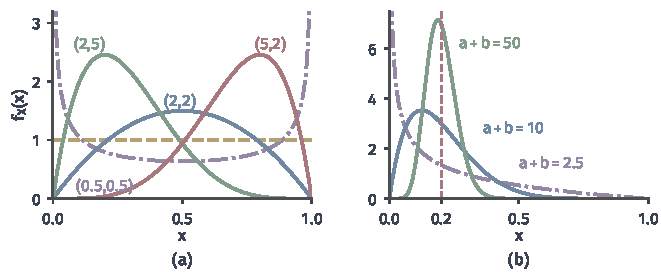
\includegraphics[width=112mm]{figures/07-probability/01-elementary-probability/matplotlib/cdist-beta-shapes/figure.pdf}
  \caption{Beta分布。(a)参数$(a,b)$为$(0.5,0.5)$（紫，U形）、$(1,1)$（黄色虚线，均匀分布）、$(2,2)$（蓝）、$(2,5)$（绿）、$(5,2)$（红）。(b)期望固定为$0.2$（红色虚线），$a+b=2.5,10,50$。}
  \label{fig:cdist-beta-shapes}
\end{BookInlineFigure}

以$X\sim\operatorname{Beta}(2,8)$描述各批次的次品比例，期望为$0.2$，方差约$0.0145$，标准差约$0.12$。由式~\eqref{eq:cdist-beta-gamma}，$\mathrm{B}(2,8)=1!\,7!/9!=1/72$。某批次比例超过$0.4$的概率为
\[
  \mathbb{P}(X>0.4)=72\int_{0.4}^{1}x(1-x)^{7}\,\mathrm{d}x .
\]
令$u=1-x$，积分化为
\[
  \int_0^{0.6}(1-u)u^{7}\,\mathrm{d}u=\frac{0.6^{8}}{8}-\frac{0.6^{9}}{9}\approx0.000980,
\]
乘以$72$得$\mathbb{P}(X>0.4)\approx0.0705$。

Beta分布描述的是一个比例的分布，与二项分布描述的次品个数是两回事：前者连续地取$(0,1)$中的值，后者在给定比例下数个数。多个比例同时变化、总和为一的情形，由第~\ref{chap:multivariate-distributions}章的Dirichlet分布推广；那里还会说明，两个相互独立、率相同的Gamma变量中，一个占两者之和的比例服从Beta分布。

\subsection{Student t分布}
\label{sec:cdist-t}

高斯模型的尾部衰减得太快：偏离$5$个标准差的概率不到$10^{-6}$。如果测量偶尔受到较大的干扰，这样的偏离会比高斯模型预言的多得多。我们想要一个仍然对称、钟形，但尾部只按幂函数衰减的密度。

把$\mathrm{e}^{-z^{2}/2}$换成$(1+z^{2}/\nu)^{-(\nu+1)/2}$就能做到。$z$很大时它与$\lvert z\rvert^{-(\nu+1)}$同阶，衰减比指数慢得多；$\nu$越大，它越像$\mathrm{e}^{-z^{2}/2}$。先算归一化常数。

\begin{lemma}[t密度的归一化]
\label{lem:cdist-t-normalization}
对$\nu>0$，
\begin{equation}
  \int_{-\infty}^{\infty}\Bigl(1+\frac{z^{2}}{\nu}\Bigr)^{-(\nu+1)/2}\mathrm{d}z
  =\sqrt\nu\,\mathrm{B}\Bigl(\frac12,\frac\nu2\Bigr)
  =\frac{\sqrt{\nu\pi}\,\Gamma(\nu/2)}{\Gamma((\nu+1)/2)} .
  \label{eq:cdist-t-normalization}
\end{equation}
\end{lemma}

\begin{proof}
被积函数是偶函数，只算$z>0$的一半再乘以$2$。令$y=z^{2}/\nu$，则$z=\sqrt{\nu y}$，并且
\[
  \mathrm{d}z=\frac{\sqrt\nu}{2\sqrt y}\,\mathrm{d}y .
\]
于是
\[
  2\int_0^{\infty}\Bigl(1+\frac{z^{2}}{\nu}\Bigr)^{-\frac{\nu+1}{2}}\mathrm{d}z
  =\sqrt\nu\int_0^{\infty}y^{-1/2}(1+y)^{-\frac{\nu+1}{2}}\,\mathrm{d}y .
\]

再令$y=t/(1-t)$，$0<t<1$。此时$1+y=1/(1-t)$，$\mathrm{d}y=\mathrm{d}t/(1-t)^{2}$，被积函数中$t$的幂次为$-1/2$，$1-t$的幂次为
\[
  \frac12+\frac{\nu+1}{2}-2=\frac\nu2-1 .
\]
所以右端的积分等于$\mathrm{B}(1/2,\nu/2)$。最后由式~\eqref{eq:cdist-beta-gamma}和$\Gamma(1/2)=\sqrt\pi$得到第二个等号。
\end{proof}

\begin{definition}[Student t分布]
\label{def:cdist-t}
设$\nu>0$，$\mu\in\mathbb{R}$，$s>0$，记
\begin{equation}
  c_\nu=\frac{\Gamma((\nu+1)/2)}{\sqrt{\nu\pi}\,\Gamma(\nu/2)} .
  \label{eq:cdist-t-constant}
\end{equation}
若随机变量$X$的密度为
\begin{equation}
  f_X(x)=\frac{c_\nu}{s}\Bigl(1+\frac{(x-\mu)^{2}}{\nu s^{2}}\Bigr)^{-(\nu+1)/2},\qquad x\in\mathbb{R},
  \label{eq:cdist-t-density}
\end{equation}
则称$X$服从自由度为$\nu$、位置为$\mu$、尺度为$s$的\term{Student t分布}（Student's t distribution），记作$X\sim t_{\nu}(\mu,s^{2})$。$\mu=0$、$s=1$时称为标准t分布，记作$t_{\nu}$。
\end{definition}

由引理~\ref{lem:cdist-t-normalization}，标准t密度的积分为一；一般情形是$\mu+sT$（$T\sim t_\nu$）的密度，由引理~\ref{lem:cdist-location-scale}，积分也为一。参数$\nu$称为\term{自由度}（degrees of freedom），它是形状参数，控制尾部的厚薄。

\paragraph{矩的存在条件}
t分布与前面各模型最大的不同在于矩可能不存在。对标准t变量$T$，当$\lvert z\rvert\geq\sqrt\nu$时，$z^{2}/\nu\leq1+z^{2}/\nu\leq2z^{2}/\nu$，所以密度被夹在$\lvert z\rvert^{-(\nu+1)}$的两个常数倍之间：
\[
  c_\nu\Bigl(\frac{2}{\nu}\Bigr)^{-\frac{\nu+1}{2}}\lvert z\rvert^{-(\nu+1)}
  \leq c_\nu\Bigl(1+\frac{z^{2}}{\nu}\Bigr)^{-\frac{\nu+1}{2}}
  \leq c_\nu\,\nu^{\frac{\nu+1}{2}}\lvert z\rvert^{-(\nu+1)}.
\]

于是对$r>0$，$\mathbb{E}\lvert T\rvert^{r}$的有限与否取决于$\int_{\sqrt\nu}^{\infty}z^{r-\nu-1}\,\mathrm{d}z$，由反常积分的比较判别，它恰在$r<\nu$时收敛。结论是
\begin{equation}
  \mathbb{E}\lvert T\rvert^{r}<\infty\iff r<\nu .
  \label{eq:cdist-t-moment-existence}
\end{equation}
所以$\nu>1$时期望存在，由对称性等于$0$；$\nu>2$时方差有限；$\nu\leq1$时期望不存在。自由度越小，存在的矩越少。

\paragraph{期望与方差}
设$\nu>2$。计算$\mathbb{E}[T^{2}]$用的代换与引理~\ref{lem:cdist-t-normalization}相同，只是被积函数多了因子$z^{2}=\nu y$，$y$的幂次从$-1/2$变成$1/2$。逐步代换后，$t$的幂次为$1/2$，$1-t$的幂次为$\nu/2-2$，于是
\[
  \int_{-\infty}^{\infty}z^{2}\Bigl(1+\frac{z^{2}}{\nu}\Bigr)^{-\frac{\nu+1}{2}}\mathrm{d}z
  =\nu^{3/2}\,\mathrm{B}\Bigl(\frac32,\frac\nu2-1\Bigr),
\]
其中$\nu/2-1>0$正是$\nu>2$的条件。

除以式~\eqref{eq:cdist-t-normalization}的归一化常数，再用式~\eqref{eq:cdist-beta-gamma}把Beta函数化成Gamma函数，分子分母中的$\Gamma((\nu+1)/2)$约去：
\[
  \mathbb{E}[T^{2}]=\nu\,\frac{\Gamma(3/2)\,\Gamma(\nu/2-1)}{\Gamma(1/2)\,\Gamma(\nu/2)}
  =\nu\cdot\frac12\cdot\frac{1}{\nu/2-1}=\frac{\nu}{\nu-2},
\]
这里用了$\Gamma(3/2)=\frac12\Gamma(1/2)$和$\Gamma(\nu/2)=(\nu/2-1)\Gamma(\nu/2-1)$。

由引理~\ref{lem:cdist-location-scale}，对$X\sim t_{\nu}(\mu,s^{2})$，
\begin{equation}
  \mathbb{E}[X]=\mu\quad(\nu>1),\qquad \operatorname{Var}(X)=s^{2}\frac{\nu}{\nu-2}\quad(\nu>2).
  \label{eq:cdist-t-moments}
\end{equation}
$1<\nu\leq2$时期望为$\mu$而方差为无穷大。尺度$s$不是标准差：$\nu=3$时标准差是$\sqrt3\,s$，$\nu=5$时是$\sqrt{5/3}\,s$。

\paragraph{Cauchy分布}
$\nu=1$的情形单独称为\term{Cauchy分布}（Cauchy distribution）。此时$c_1=\Gamma(1)/(\sqrt\pi\,\Gamma(1/2))=1/\pi$，标准情形的密度为
\begin{equation}
  f(x)=\frac{1}{\pi(1+x^{2})},\qquad x\in\mathbb{R}.
  \label{eq:cdist-cauchy-density}
\end{equation}
它关于$0$对称，但期望不存在。正半轴上的积分发散：
\[
  \int_0^{R}\frac{x}{\pi(1+x^{2})}\,\mathrm{d}x=\frac{1}{2\pi}\ln(1+R^{2})\to\infty .
\]
负半轴同样发散，正负两部分都是无穷大，按第~\ref{chap:random-variable-moments}章的规定，期望没有定义。

对称性诱使人说“期望是$0$”，可以用不对称的截断看出这为何不行。把积分区间取成$[-R,cR]$，$c>0$，则
\[
  \int_{-R}^{cR}\frac{x}{\pi(1+x^{2})}\,\mathrm{d}x=\frac{1}{2\pi}\ln\frac{1+c^{2}R^{2}}{1+R^{2}}\to\frac{\ln c}{\pi}\qquad(R\to\infty).
\]
对称截断（$c=1$）给出$0$，$c=2$给出$\ln2/\pi\approx0.221$，$c=1/2$给出$-0.221$。极限依赖于截断的方式，说明这里没有一个确定的“平均位置”，见图~\ref{fig:cdist-cauchy-truncation}。

\begin{BookInlineFigure}
  \centering
  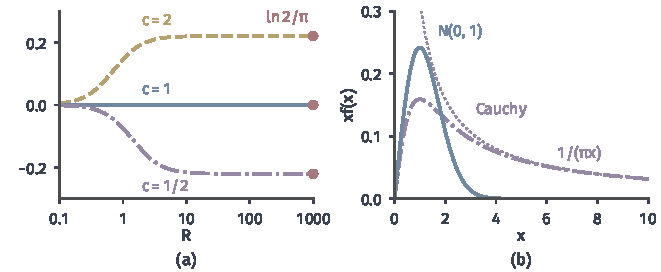
\includegraphics[width=112mm]{figures/07-probability/01-elementary-probability/matplotlib/cdist-cauchy-truncation/figure.pdf}
  \caption{Cauchy分布的期望不存在。(a)截断积分$\int_{-R}^{cR}xf(x)\,\mathrm{d}x$随$R$的变化，$c=2$（黄）、$1$（蓝）、$1/2$（紫），横轴为对数刻度，红点为三个不同的极限$\ln c/\pi$。(b)$xf(x)$：Cauchy分布（紫）按$1/(\pi x)$（紫色点线）衰减，积分发散；$\mathcal{N}(0,1)$（蓝）很快衰减到零。}
  \label{fig:cdist-cauchy-truncation}
\end{BookInlineFigure}

Cauchy分布的位置要用中位数描述。标准情形的分布函数为$F(x)=\frac12+\frac1\pi\arctan x$，中位数是$0$，上下四分位数是$\pm1$。所以$t_1(\mu,s^{2})$的中位数是$\mu$，尺度$s$恰好是四分位距的一半：$\mu$是对称中心与中位数，但不是期望。

\paragraph{与高斯分布的关系}
$\nu\to\infty$时t密度趋于标准高斯密度。函数部分取对数，与定理~\ref{thm:cdist-binomial-poisson}证明中的方法相同：
\[
  -\frac{\nu+1}{2}\ln\Bigl(1+\frac{z^{2}}{\nu}\Bigr)\to-\frac{z^{2}}{2}.
\]
式~\eqref{eq:cdist-t-constant}中的常数$c_\nu$趋于$1/\sqrt{2\pi}\approx0.3989$，证明需要Gamma函数的渐近公式，这里只列出数值：$\nu=1,3,10,30,100$时依次约为$0.3183$、$0.3676$、$0.3891$、$0.3956$、$0.3979$。

图~\ref{fig:cdist-t-tails}(a)中$\nu=30$的t密度已与高斯密度几乎重合，差别集中在尾部。图~\ref{fig:cdist-t-tails}(b)用对数纵轴画出双侧尾概率：$\mathbb{P}(\lvert T\rvert>3)$在高斯、$t_3$和Cauchy情形分别约为$0.0027$、$0.0577$、$0.2048$，差了两个数量级。

\begin{BookInlineFigure}
  \centering
  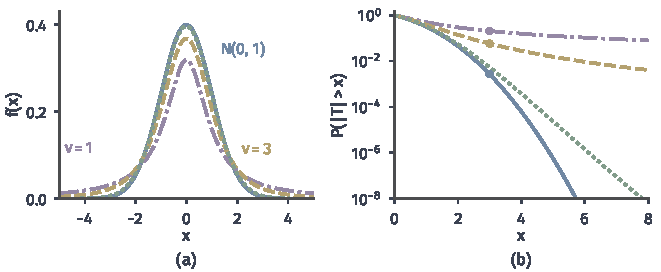
\includegraphics[width=112mm]{figures/07-probability/01-elementary-probability/matplotlib/cdist-t-tails/figure.pdf}
  \caption{t分布与高斯分布。(a)标准高斯（蓝）与$\nu=1$（紫）、$\nu=3$（黄）、$\nu=30$（绿色点线，几乎与蓝线重合）的标准t密度。(b)双侧尾概率$\mathbb{P}(\lvert T\rvert>x)$，纵轴为对数刻度，圆点为$x=3$处的值；高斯尾部按$\mathrm{e}^{-x^{2}/2}$下降，t分布按幂函数下降。}
  \label{fig:cdist-t-tails}
\end{BookInlineFigure}

t分布还可以由高斯变量构造：设$Z\sim\mathcal{N}(0,1)$与$U\sim\chi^{2}_{\nu}$相互独立，则$Z/\sqrt{U/\nu}\sim t_\nu$。这相当于给高斯变量配上一个随机的尺度，尺度偶尔变得很大，就产生了厚尾。这个比值的分布在第~\ref{chap:random-variable-transformations}章推导，多个分量共享同一随机尺度的情形见第~\ref{chap:multivariate-distributions}章。

\subsection{Laplace分布}
\label{sec:cdist-laplace}

另一种加厚尾部的办法是把高斯密度指数中的平方换成绝对值。$\mathrm{e}^{-\lvert x\rvert}$在原点有一个尖角，尾部按指数而不是按$\mathrm{e}^{-x^{2}/2}$衰减：比高斯厚，但仍比任何幂函数薄。

\begin{definition}[Laplace分布]
\label{def:cdist-laplace}
设$\mu\in\mathbb{R}$，$b>0$。若随机变量$X$的密度为
\begin{equation}
  f_X(x)=\frac{1}{2b}\exp\Bigl(-\frac{\lvert x-\mu\rvert}{b}\Bigr),\qquad x\in\mathbb{R},
  \label{eq:cdist-laplace-density}
\end{equation}
则称$X$服从参数为$\mu,b$的\term{Laplace分布}（Laplace distribution），记作$X\sim\operatorname{Laplace}(\mu,b)$。
\end{definition}

$\mu$是位置参数，$b$是尺度参数。标准情形$\mu=0$、$b=1$的密度是$\frac12\mathrm{e}^{-\lvert z\rvert}$，分成正负两半各积一次指数，每半的积分是$1/2$，总和为一。右半边恰好是率为$1$的指数密度的一半，这也是它又叫双指数分布的原因：给定$X>\mu$，$X-\mu$服从$\operatorname{Exp}(1/b)$。

\paragraph{期望与方差}
对标准情形$Z$，绝对矩可以用Gamma函数算出：
\[
  \mathbb{E}\lvert Z\rvert^{k}=2\int_0^{\infty}z^{k}\cdot\frac12\mathrm{e}^{-z}\,\mathrm{d}z=\Gamma(k+1)=k!,\qquad k=0,1,2,\dots .
\]
所有阶的矩都有限。密度对称，所以$\mathbb{E}[Z]=0$，$\operatorname{Var}(Z)=\mathbb{E}[Z^{2}]=2$。由引理~\ref{lem:cdist-location-scale}，
\begin{equation}
  \mathbb{E}[X]=\mu,\qquad \operatorname{Var}(X)=2b^{2}.
  \label{eq:cdist-laplace-moments}
\end{equation}
标准差为$\sqrt2\,b$，尺度$b$同样不是标准差。四阶中心矩为$24b^{4}$，峰度为$24b^{4}/(2b^{2})^{2}=6$，比高斯分布的$3$大$3$。

尾概率也有简单的形式。分两侧积分，
\begin{equation}
  \mathbb{P}(\lvert X-\mu\rvert>t)=\mathrm{e}^{-t/b},\qquad t\geq0 .
  \label{eq:cdist-laplace-tail}
\end{equation}

\paragraph{与高斯分布的比较}
比较形状要在相同的方差下进行，否则只是尺度不同。取方差都为$1$：$\mathcal{N}(0,1)$与$\operatorname{Laplace}(0,1/\sqrt2)$。两者的峰值分别是$1/\sqrt{2\pi}\approx0.399$和$1/\sqrt2\approx0.707$，Laplace分布的中心更尖。

两条密度曲线在$\lvert x\rvert\approx0.49$和$\lvert x\rvert\approx2.34$处相交。中间一段（$0.49<\lvert x\rvert<2.34$）高斯密度更高，两端Laplace密度更高，所以Laplace分布同时有更尖的中心、更薄的“肩部”和更厚的尾部。方差相同，质量的分布方式却不同。

到远处差别更明显。由式~\eqref{eq:cdist-laplace-tail}，偏离超过$3$个标准差的概率为$\mathrm{e}^{-3\sqrt2}\approx0.0144$，是高斯分布$0.0027$的五倍多；超过$5$个标准差时，Laplace约为$8.5\times10^{-4}$，高斯不到$6\times10^{-7}$。在对数纵轴上，Laplace的对数密度在$x>0$一侧是直线，高斯的是向下弯的抛物线，见图~\ref{fig:cdist-laplace-normal}(b)。

\begin{BookInlineFigure}
  \centering
  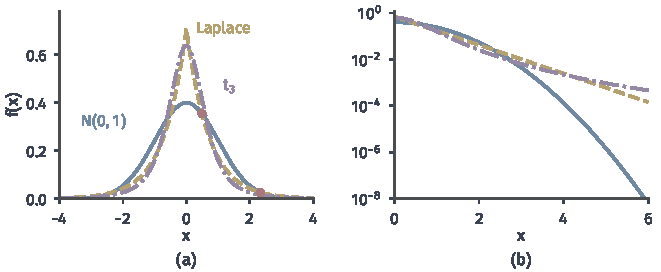
\includegraphics[width=112mm]{figures/07-probability/01-elementary-probability/matplotlib/cdist-laplace-normal/figure.pdf}
  \caption{方差都为$1$的三种对称分布：$\mathcal{N}(0,1)$（蓝）、$\operatorname{Laplace}(0,1/\sqrt2)$（黄）和尺度为$1/\sqrt3$的$t_3$（紫）。(a)密度，红点为高斯与Laplace密度在右侧的两个交点。(b)$x\geq0$部分的对数密度。}
  \label{fig:cdist-laplace-normal}
\end{BookInlineFigure}

图中还画了方差同为$1$的$t_3$分布。它的中心与Laplace相近，在$3$个标准差处的双侧尾概率约为$0.0138$，也与Laplace相当；到$5$个标准差处约为$0.0032$，已是Laplace的近四倍，因为幂函数尾部最终总比指数尾部厚。Laplace分布有全部阶的矩，$t_3$的四阶矩却是无穷大。只看方差，这三个分布无法区分。

Laplace变量也可以由两个独立的指数变量之差得到，这在第~\ref{chap:random-variable-transformations}章证明。多元推广有好几种不同的构造，它们的边缘都是Laplace分布，依赖结构却不相同，第~\ref{chap:multivariate-distributions}章会分别说明。
